\documentclass[12pt, a4paper]{report}
\usepackage{parskip}
\usepackage[utf8]{inputenc}
\usepackage{fancyhdr}
\usepackage{pifont}
\usepackage{bibentry}
\makeatletter\let\saved@bibitem\@bibitem\makeatother
\usepackage{hyperref}
\makeatletter\let\@bibitem\saved@bibitem\makeatother
\usepackage{tikz}
\usetikzlibrary{trees,positioning,shapes,shadows,arrows}

\newcommand{\stars}[1]{{\count0=#1 \loop \ifnum\count0>0 \advance\count0 by -1 \ding{80}\repeat}}
\newcommand{\record}[2]{\newpage\section*{\href{/library/#1.pdf}{#1}}\bibentry{#1}\fancyhf{}\lhead{#1}\rhead{#2}\par\bigbreak}
\pagenumbering{gobble}
\pagestyle{fancy}
\title{Reading Diary}
\author{Lakshan Bernard}
\tikzset{mystyle/.style={fill=blue}}
\date{\today}




\begin{document}

\begin{titlepage}\maketitle\end{titlepage}
\nobibliography{references.bib}
\bibliographystyle{ieeetr}
\tableofcontents{}


\chapter{Stability}

\record{hatziargyriou2020stability}{??/??/2020}
Write a summary of the paper...

\record{ghanavati2016identifying}{??/??/2020}
Prior research has shown that autocorrelation and variance in voltage measurements tend to increase as power systems approach instability. This paper seeks to identify the conditions under which these statistical indicators provide reliable early warning of instability in power systems. First, the paper derives and validates a semi-analytical method for quickly calculating the expected variance and autocorrelation of all voltages and currents in an arbitrary power system model. Building on this approach, the paper describes the conditions under which filtering can be used to detect these signs in the presence of measurement noise. Finally, several experiments show which types of measurements are good indicators of proximity to instability for particular types of state changes. For example, increased variance in voltages can reliably indicate both proximity to a bifurcation and the location of increased stress. On the other hand, growth of autocorrelation in certain line currents is related less to a specific location of stress but, rather, is a reliable indicator of stress occurring somewhere in the system; in particular, it would be a clear indicator of approaching instability when many nodes in an area are under stress.

\record{meegahapola2020review}{30/06/2020}
\stars{5} This is a recent review paper on oscillatory stability. It contain 100+ references and covers established theory and open research questions relating to Power Electronic Converter (PEC) renewable energy generation.\par
\textbf{Applications:} Using synchrophasors for analysing oscillatory stability is well established in literature but further work is required to cope with PEC induced oscillations. The challenges introduced by PEC generation include: Frequency regulation/control; Voltage control; Oscillatory stability; Power quality (harmonics, flicker, etc.). \par
Over the past few years, research has been conducted into how PEC devices impact the damping performance of the power grid. Types of PEC studied include: Doubly Fed Induction Generator (DFIG); Permanent Magnet Synchronous Generator (PMSG); Non-linear loads such as Variable Speed Drive (VSD); Switch mode power supply; and Light Emitting Diode (LED) drives.\par
\textbf{Synchrophasors vs SCADA:} For this type of research, synchrophasors have superceded the capability of SCADA systems, primarily due to their high accuracy and high speed data transfer capabilities. The broad categories of research in synchrophasors can be divided as follows:\par
\begin{center}\resizebox{!}{4.5cm}{
	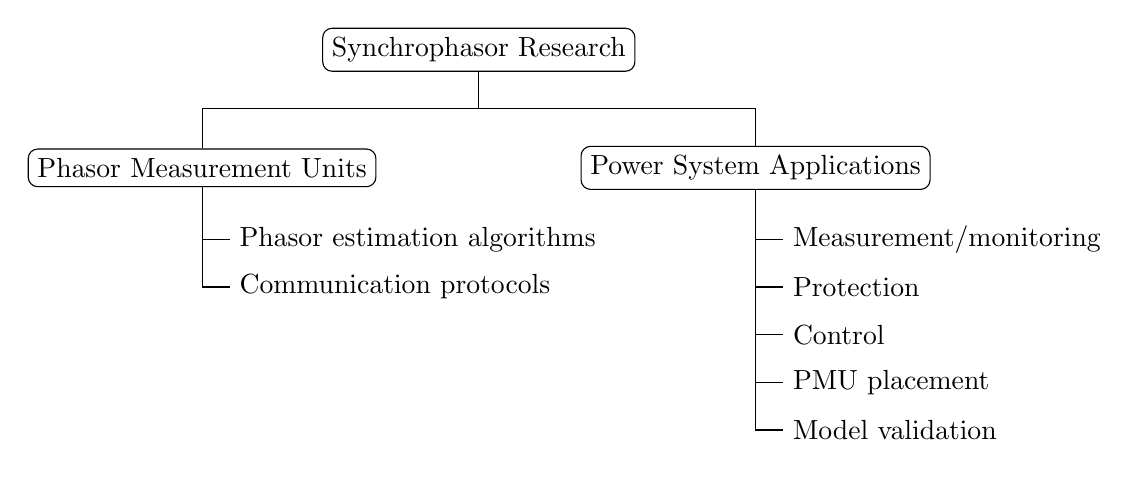
\begin{tikzpicture}[
  		leaf/.style={},
  		root/.style={rectangle,draw,fill=white,rounded corners=.8ex},
  		grandchild/.style={grow=down,xshift=1em,anchor=west,
    		edge from parent path={(\tikzparentnode.south) |- (\tikzchildnode.west)}},
  		level 1/.style={sibling distance=20em}]
    		% Parent
      		\node[root]{Synchrophasor Research}
    			[edge from parent fork down]
    		% Children and grandchildren
    			child{node[root]{Phasor Measurement Units}
      				child[grandchild,level distance=6ex] {node[leaf]{Phasor estimation algorithms}}
				child[grandchild,level distance=10ex] {node[leaf]{Communication protocols}}}
    			child {node[root]{Power System Applications}
      				child[grandchild,level distance=6ex] {node[leaf]{Measurement/monitoring}}
      				child[grandchild,level distance=10ex] {node[leaf]{Protection}}
			      	child[grandchild,level distance=14ex] {node[leaf]{Control}}
			      	child[grandchild,level distance=18ex] {node[leaf]{PMU placement}}
			      	child[grandchild,level distance=22ex] {node[leaf]{Model validation}}};
	\end{tikzpicture}
}\end{center}
This review also includes a nice summary of definitions relating to PMUs. Phase Locked Loop (PLL) is the fastest estimation technique but accuracy decreases under harmonic distortions. Quadrature demodulation is described as very accurate and DFT based methods are most commercially available.\par
Individual PMUs feed into a Phasor Data Concentrator (PDC) and large networks have multiple PDCs in a hierarchy (local$\,\to\,$regional$\,\to\,$coorporate). It is at the PDCs that real-time situational awareness algorithms (e.g. to monitor voltage stability, transient stability, oscillatory stability) are deployed. Note local PDCs have less delay but limited view of the grid, whereas the coorporate/central has a full view of the network but longer delays. The review paper did not mention the order of magnitude of these delays.\par
\textbf{Classification:} The types of power system oscillation are depicted below:
\begin{center}\resizebox{\columnwidth}{!}{
	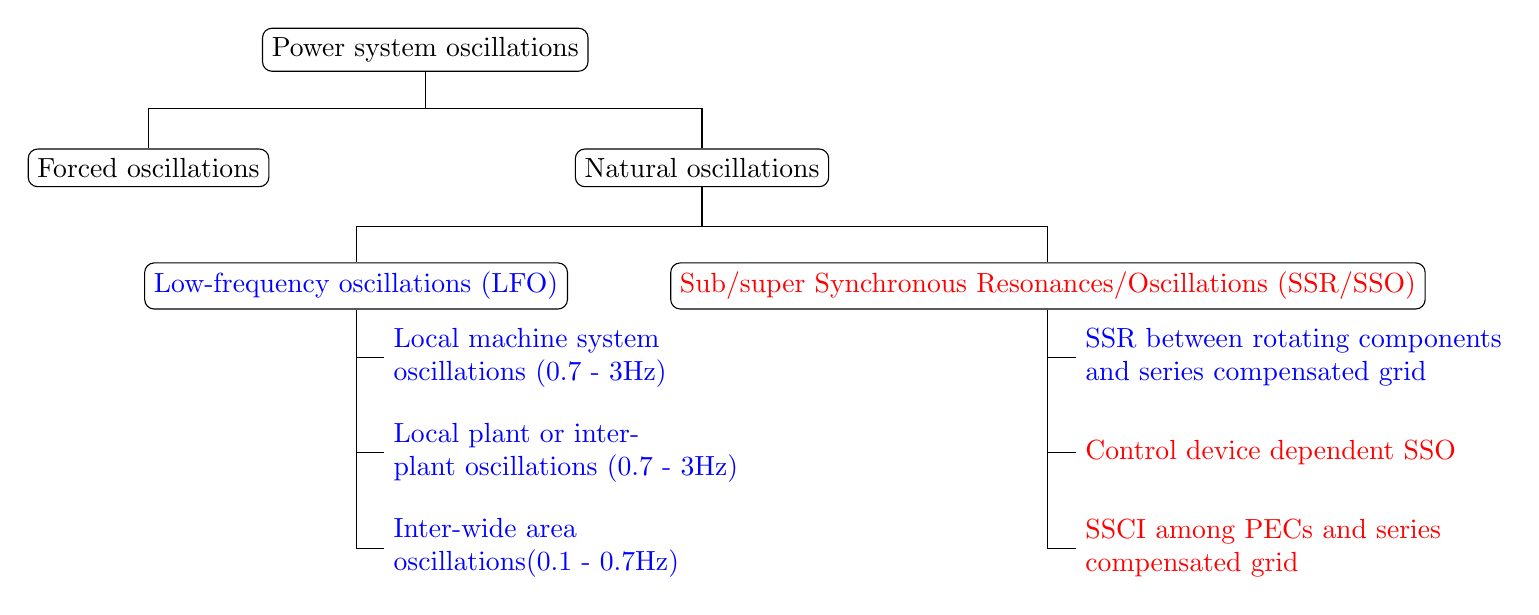
\begin{tikzpicture}[
  		leaf/.style={align=left},
  		root/.style={align=center, rectangle,draw,fill=white,rounded corners=.8ex},
  		grandchild/.style={grow=down,xshift=1em,anchor=west,
    		edge from parent path={(\tikzparentnode.south) |- (\tikzchildnode.west)}},
  		level 1/.style={sibling distance=20em},
  		level 2/.style={sibling distance=25em}]
    		% Parent
      		\node[root]{Power system oscillations}
    			[edge from parent fork down]
    		% Children and grandchildren
    			child{node[root]{Forced oscillations}}
    			child{node[root]{Natural oscillations}
      				child{node[root,text=blue]{Low-frequency oscillations (LFO)}
      					child[grandchild,level distance=6ex,text=blue] {node[leaf]{Local machine system\\ oscillations (0.7 - 3Hz)}}
      					child[grandchild,level distance=14ex,text=blue] {node[leaf]{Local plant or inter-\\ plant oscillations (0.7 - 3Hz)}}
			      		child[grandchild,level distance=22ex,text=blue] {node[leaf]{Inter-wide area\\ oscillations(0.1 - 0.7Hz)}}}
			      	child{node[root,text=red]{Sub/super Synchronous Resonances/Oscillations (SSR/SSO)}
      					child[grandchild,level distance=6ex,text=blue] {node[leaf]{SSR between rotating components\\ and series compensated grid}}
      					child[grandchild,level distance=14ex,text=red] {node[leaf]{Control device dependent SSO}}
			      		child[grandchild,level distance=22ex,text=red] {node[leaf]{SSCI among PECs and series \\ compensated grid}}}};
	\end{tikzpicture}
}\end{center}
Forced oscillations arise from cyclic oscillating sources (e.g. fluctuations of renewables). LFO involves synchronous generators and has extensively been studied. SSO/SSR was defined by the SSR working group (from the IEEE Power System and Dynamic Performance subcommittee) in 1976 and revised in 1979, 1985, 1991 and 1997. Recently, wind and solar generation is causing new types of SSO/SSR. Thus SSO/SSR is reclassified into three sub-categories:
\begin{enumerate}
	\item SSR between rotating components and series compensated grid. This includes  Induction Generator/Machine Effect (IGE/IME), Torque Amplification (TA), and Torsional Interaction (TI).
	\item Control device dependent SSO. This includes the steam/hydro against fast response controllers, and Sub Synchronous Torsional Interaction (SSTI).
	\item Sub Synchronous Control Interaction (SSCI) among PECs and series compensated grid. These are newly observed oscillations that need to be adequately dampened. 
\end{enumerate}
\textbf{Monitoring methods}: Traditionally, time domain simulations were used for modal analysis, however, this is no longer practical because: increased quantity of PECs has complicated dynamic models with time-varying parameters, `black-box' controllers, and large computational burden for real time applications. For example, model-based approaches were unable to identify the oscillation in the 1996 USA blackout. The future is using PMUs for real time monitoring of power system dynamics.\par
The first group of methods aim to \emph{estimate the oscillation mode and/or the oscillation mode shape}. The typical data collected by the PMU is called ambient, while the post-fault data is called ringdown.
\begin{center}\resizebox{\textwidth}{!}{
	\begin{tabular}{ |l|c|c|c|c| } 
		\hline
		\textbf{Method} & \textbf{Mode} & \textbf{Shape} & \textbf{Data}  \\\hline 
		Stochastic subspace system identification 	& \textcolor{blue}{Y}	& \textcolor{blue}{Y} 		& Both		\\\hline
		Prony analysis					& \textcolor{blue}{Y}	& \textcolor{blue}{Y}		& Ringdown	\\\hline
		Matrix pencil					& \textcolor{blue}{Y} 	& \textcolor{blue}{Y}		& Ringdown	\\\hline
		Phase locked loop method			& \textcolor{blue}{Y} 	& \textcolor{blue}{Y}		& Ringdown	\\\hline
		Frequency domain decomposition			& \textcolor{blue}{Y}	& \textcolor{blue}{Y}		& Ambient	\\\hline
		ARMAX model					& \textcolor{blue}{Y}	& \textcolor{blue}{Y}		& Ambient 	\\\hline
		Continuous modal parameter estimator		& \textcolor{red}{N}	& \textcolor{blue}{Y}		& Ringdown	\\\hline
		Principal component analysis			& \textcolor{red}{N}	& \textcolor{blue}{Y}		& Ringdown	\\\hline
		Moment matching method				& \textcolor{red}{N}	& \textcolor{blue}{Y}		& Ringdown	\\\hline
		Kalman filtering				& \textcolor{red}{N}	& \textcolor{blue}{Y}		& Ringdown	\\\hline
		Cross spectrum analysis				& \textcolor{red}{N}	& \textcolor{blue}{Y}		& Ambient	\\\hline
		Channel matching method				& \textcolor{red}{N}	& \textcolor{blue}{Y}		& Ambient	\\\hline
		Transfer function				& \textcolor{red}{N}	& \textcolor{blue}{Y}		& Ambient 	\\\hline
		Minimal realisation				& \textcolor{blue}{Y}	& ?				& Ringdown 	\\\hline
		Eigensystem realisation				& \textcolor{blue}{Y}	& ?				& Ringdown	\\\hline
		Fourier transformation				& \textcolor{blue}{Y}	& ?				& Ringdown	\\\hline
		Hilbert-Hung transformation			& \textcolor{blue}{Y}	& ?				& Ringdown	\\\hline
		Wavelet transformation				& \textcolor{blue}{Y}	& ?				& Ringdown	\\\hline
		Variable projection				& \textcolor{blue}{Y}	& ?				& Ringdown	\\\hline
		Spectral analysis				& \textcolor{blue}{Y}	& ?				& Ambient	\\\hline
		Yule-Walker method				& \textcolor{blue}{Y}	& ?				& Ambient	\\\hline
		LMS adaptive filtering				& \textcolor{blue}{Y}	& ?				& Both		\\\hline
		Robust recursive least squares			& \textcolor{blue}{Y}	& ?				& Both		\\\hline
	\end{tabular}
}\end{center}
Even though the stochastic subspace system identification can estimate the mode and the mode shape with both types of data, it has a high computational cost. The key improvements to this group of methods are: 1) past research has exclusively targeted LFO - the new oscillation modes (e.g. power resonance caused by renewables interaction with voltage source converters and  HVDC controllers) are still to be solved; 2) there is interest in algorithms that work for both ringdown and ambient data; 3) most research does not consider data cleanliness issues (e.g. how to cope with missing packets); 4) the oscillation mode shapes are not enough to identify the source of the oscillation; and 5) these methods do not show how damping is distributed throughout the grid - hence they can only be used for monitoring purposes.\par
The second class of methods to monitor oscillations are called \emph{energy flow tracking}. The idea is to calculate the damping torque coefficent $K_D(f)$ for each device in the network. For a Single Machine Infinite Bus (SMIB) there is rigorous theory justifying how to calculate the $K_D(f)$ using the cross-energy spectral density and angular velocity of the terminal voltage. Recently there is a renewed interest in this type of method because: 1) it is computationally efficient; 2) the source and cause of the oscillation is identified by having negative $K_D(f)$; 3) the theory is general enough that it can deal with a wide frequency of oscillations - not just LFO. The room for improvement is that the theory has still not been extended from SMIB to a real power system so this method is currently restricted to local application. It is unclear how to extend this theory to find the system oscillatory stability margin.\par
\textbf{Non-fundamental phasors:} Originally, PMUs were designed to monitor the fundamental phasor. When the reporting rate is high (e.g. 100Hz) it is possible to analyse variations in the fundamental phasor to find the presence of sub synchronous oscillations. The is current research interest in algorithms that can extract the frequency, damping coefficient, amplitude and phase angle of any sub synchronous oscillations present. There are four standard methods: Prony, Hankel total least squares, eigensystem realisation and matrix pencil. All these methods feature a data matrix which is processed and end with a least square solution. It is also found that the Fourier transform can be used to extract the frequency and damping of sub synchronous oscillations.\par
During sub-synchronous oscillation based events, there can also be super synchronous interharmonics. Even with a reporting rate of 100Hz, these interharmonics cannot be identified by solely analysing the fundamental phasor. Instead, the conventional DFT based phasor estimation algorithm inside the PMUs should be updated. This is also an active field of research including Synchronised Measurement Devices (SMD) and the Improved Iterative Taylor Fourier Multifrequency (I2TFM).\par
\textbf{Damping systems:} When poorly damped, oscillatory modes (esp. LFO inter-area) limit the power transfer along lines which can cause a failure in the system. The majority of the literature tackles inter-area oscillations (viz. sub synchronous oscillations).\par
The first technique is to treat the inadequate damping of oscillations as a small signal problem and use a linearised model of the system. Traditionally, this involved a Power System Stabiliser (PSS) that provides a control signal to an Automatic Voltage Regulator (AVR). The drawbacks of this approach are: 1) validity of linear model around multiple operating points; 2) robustness of the designed controller to work under multiple operating conditions; 3) model uncertainities; 4) computational complexities; and 5) simultaneously damping local and inter-area oscillatory modes.\par
The majority of techniques are called \emph{robust and adaptive controllers} because they handle model uncertainities and adaptively update to cope with a variety of operating conditions. State of the art techniques include: the $H_\infty$ controller; multiagent $H_\infty$ controller; mixed $H_2/H_\infty$ controller; dual Youla parameterisation based adaptive controller; and the multi-polytopic adaptive controller. Consideration must also be given to communication delay arising from remote signal - this is taken in consideration by the: networked predictive control approach; phasor power oscillation damping controller; enhanced adaptive phasor power oscillation damping controller; Smith predictor based $H_\infty$ controller; recurrent neural network based controller; stochastic subspace indentification based controllers.\par
The final category of synchrophasor based damping control mentioned uses Flexible AC Transmission System (FACTS) devices such as Thyristor Controlled Series Capacitor (TCSC) and Static VAR Compensators (SVCs).\par
\textbf{Real power grids:} A comparison is made between: Statnett Power Oscillation Monitoring System (Nordic Energy Network), SGCC WAMS Platform (China), Swissgrid WAMS (Swissgrid), Southern California Edison Company (Southern California), Manitoba Hydro (Manitoba) and Tennessee Valley (Knoxville Tennessee). These example show that the monitorred oscillatory modes are \textless 2 Hz hence corresponds to the LFO. The Statnett Power Oscillation Monitoring System is highlighted since it was implemented in parallel with SCADA data (fault recorders). It is reliable with communication latencies upto 300ms.\par
\textbf{Big data:} Synchrophasor data is saved on databases. Big data has large volume, variety and velocity - thus covers synchrophasor databases. The most common big data technique used on synchrophasor databases is data mining, in particular classification and regression approaches are most common. Typical application include Dynamic Stability Assessment (DSA); instability prediction; state estimation; and protection. Parallel processing is also essential to deal with synchrophasor data streams, so there is active research in `upgrading' conventional algorithms by finding more efficient decompositions, exploiting sparsity, splitting the data into smaller blocks, etc.\par
The application for dynamic event detection is also highlighted. One algorithm consisted of using Finite Impulse Response (FIR) filters to find line outages. Event location was also considered in a offline hierarchical clustering approach to group coherent generators. Detecting transient events has also been considered using Detrended Fluctuation Analysis.\par
Very interesting research has also been conducting in using advanced statistics on synchrophasor data. The main aim is to design statisical indices to predict stability issues in power networks. The first example uses autocorrelation and variance of bus voltages to produce early warning signs of separation events. The second example uses Linear Eigenvalue Statistics (LES) for situational awareness in power grids, especially enabling anomaly detection.
\textbf{Recommendations:} There are five main recommendations:
\begin{enumerate}
	\item Monitoring mixed oscillation issues caused by PEC, not just LFO.
	\item Extending energy flow tracking from SMIB to real power grids.
	\item Dealing with synchrophasor data cleanliness.
	\item Monitoring sub synchronous oscillations from fundamental phasor data.
	\item Use of big data for oscillatory stability monitoring.
\end{enumerate} 
 


\chapter{System Strength}

\record{gu2019review}{??/??/2020}
Synchronous generators (SGs) are still making major contributions to the re-stabilization of a power system following voltage/frequency disturbances, attributed to their inherent capability of providing system strength and inertia. However, SGs powered by fossil fuels are operating to a lesser extent and scheduled for decommissioning in the National Electricity Market (NEM) of Australia due to the accelerating increase of low bidding priced asynchronous generation of wind and solar, which leads to the reduction and even in some cases, a shortage of system strength and inertia. This paper comprehensively reviews the requirements of system strength and inertia in the NEM from an operational security perspective. Australia is the first country that established the regulation rules of system strength and inertia to accommodate issues of an emerging high penetration level of non-synchronous renewable generation.



\chapter{Example Chapter}

\record{einstein1935can}{27/06/2020}
I can write a summary of the paper here. I can write multiple paragraphs as follows. \par
The title of this page is the BibTeX key. The title itself is hyperlinked to the PDF of the paper. If the link does not work check the folder structure is consistent and perhaps try with a different PDF viewer (it works in Evince document viewer). When it comes time to cite this paper, I can quickly copy the BibTeX key into my LaTeX file without rummaging through the references.bib file. \par
Also note the bibliography entry is displayed above so that I can check the fields in the references.bib file have been entered properly. Since it contains indexable information (e.g. title, authors, year of publication, journal, etc.) we can use the search feature of the PDF viewer to find specific papers. \par
Each summary begins on a new page and the header also displays the BibTeX key on the left. On the right is the date that I read the paper. There is full control over the order the summaries are displayed by moving them around in the reading.tex file. I like to have a reverse chronological order since what I read recently is at the top. \par
Each paper can be assigned to a chapter for easy sorting. At the moment it is not possible to add a paper into two chapters simultaneously so I just choose the most appropriate chapter. Later on, I might make a HTML interface that allows assigning tags to each summary to make sorting more practical. \par
Since this a LaTeX document, it is quite easy to enter math mode to write equations, for example:
$$
\sin^2\theta + \cos^2\theta = 1
$$
It is also possible to have tables and even draw diagrams using TikZ.

\end{document}
